
\chapter{Graph}

\section{Definition Graph}


\begin{theorem}
Ein \textbf{Graph} G besteht aus einer Menge X [deren Elemente Knotenpunkte genannt werden] und einer Menge U, wobei jedem Element u $\in$ U in eindeutiger Weise ein geordnetes oder ungeordnetes Paar von [nicht notwendig verschiedenen] Knotenpunkten, x,y $\in$ X zugeordnet ist.
Ist jedem u $\in$ U ein geordnetes Paar von Knoten zugeordnet, so heißt der Graf \textbf{gerichtet}, und wir schreiben 
	$G= (X, U)$.
Die Elemente von U werden in diesem Fall als \textbf{Bögen} bezeichnet.

Ist jedem u $\in$ U ein ungeordnetes Paar von Knotenpunkten zugeordnet, so heißt der Graph \textbf{ungerichtet} und wir schreiben 
	$G=[X,U]$. 
Die Elemente von U bezeichnen wir dann als \textbf{Kanten.} \\
\cite[S. 9]{Biess09} 	%%\footnote{Bieß, Graphentheorie, S.9}\\
\end{theorem} 

\begin{figure}[h]
\centering
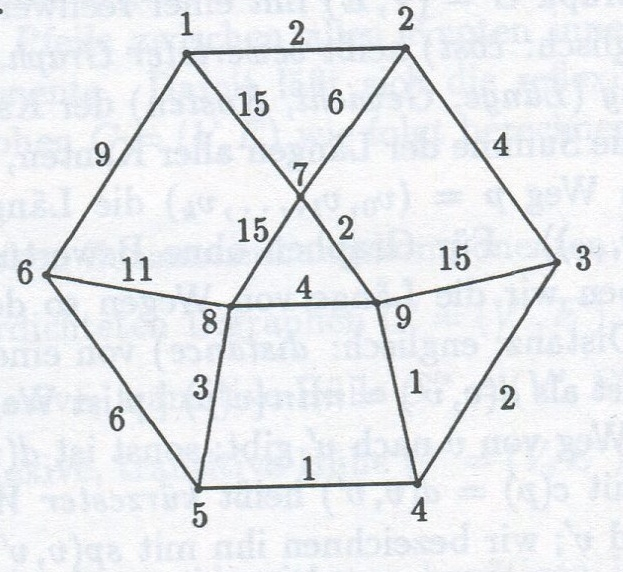
\includegraphics[width = 8cm]{./chapters/Graph.jpg}
\caption{Beispielgraph \cite[S.572 Abb. 8.18]{OttWid90}
%{\tiny (Quelle: OTTMANN, Thomas; WIDMAYER Peter: Algorithmen und Datenstrukturen, Reihe Informatik Bd. 70, Mannheim: BI-Wissenschaftsverlag, 1990, S.572 Abb. 8.18)} 
}
\label{a1}
\end{figure}


Ein gerichteter Graph, auch Digraph genannt,  besteht somit aus einer Menge aus geordneten Knotenpunkten \footnote{Ottman, Datenstrukturen und Algorithmen, S590}. Dadurch, dass diese Punkte geordnet sind, also zu jedem Element U genau ein Paar Knotenpunkte zugeordnet wird, ist eine Verlaufsrichtung festgelegt, in welcher der Graph zeigt.

Die Verbindungslinien zwischen zwei Knotenpunkten werden Kanten genannt, welchen Kosten zugeordnet sind. Diese Kosten sind im Vornherein festgelegte, nicht negative Werte. Sie sind  nicht mit der Kantenlänge zu verwechseln.

Somit kann sich eine geometrische Figur ergeben.\\

Weiterhin gibt es auch ungerichtete Graphen, welche jedoch in dieser Ausarbeitung keine Bedeutung haben und somit an dieser Stelle nicht weiter erläutert werden.
In der folgenden Arbeit wird jedoch mit anderen Bezeichnungen gearbeitet. Anstelle von der von Gieß gebrauchten Bezeichnung G=(X,U), wird G=(V,E) verwendet.



\section{Datenstrukturen zur Repräsentation von Graphen}

\textbf{Speicherung in einer Adjazenzmatrix} \\
Der Graph G=(V,E) wird in einer booleschen m*m Matrix gespeichert ($m = \sharp V$), mit 1 falls $(i,j) \in E$ und 0 falls nicht. \\
Nachteil: Dies erfordert unverhältnismäßig viel Speicher, wenn der Graph nur wenig    	  Kanten hat. Abhilfe schafft eine Zusatzmatrix, die nur bedeutsame Einträge speichert.
 Insgesamt ist eine Adjazenzmatrix aber trotzdem ineffizient bei Graphen mit wenig Kanten. 
  \footnote{OTTMANN, Thomas; WIDMAYER Peter: Algorithmen und Datenstrukturen, Reihe Informatik Bd. 70, Mannheim: BI-Wissenschaftsverlag, 1990, S.539-541, Speicherung in einer Adjazenzmatrix}\\
 

\begin{figure}[h]
\centering
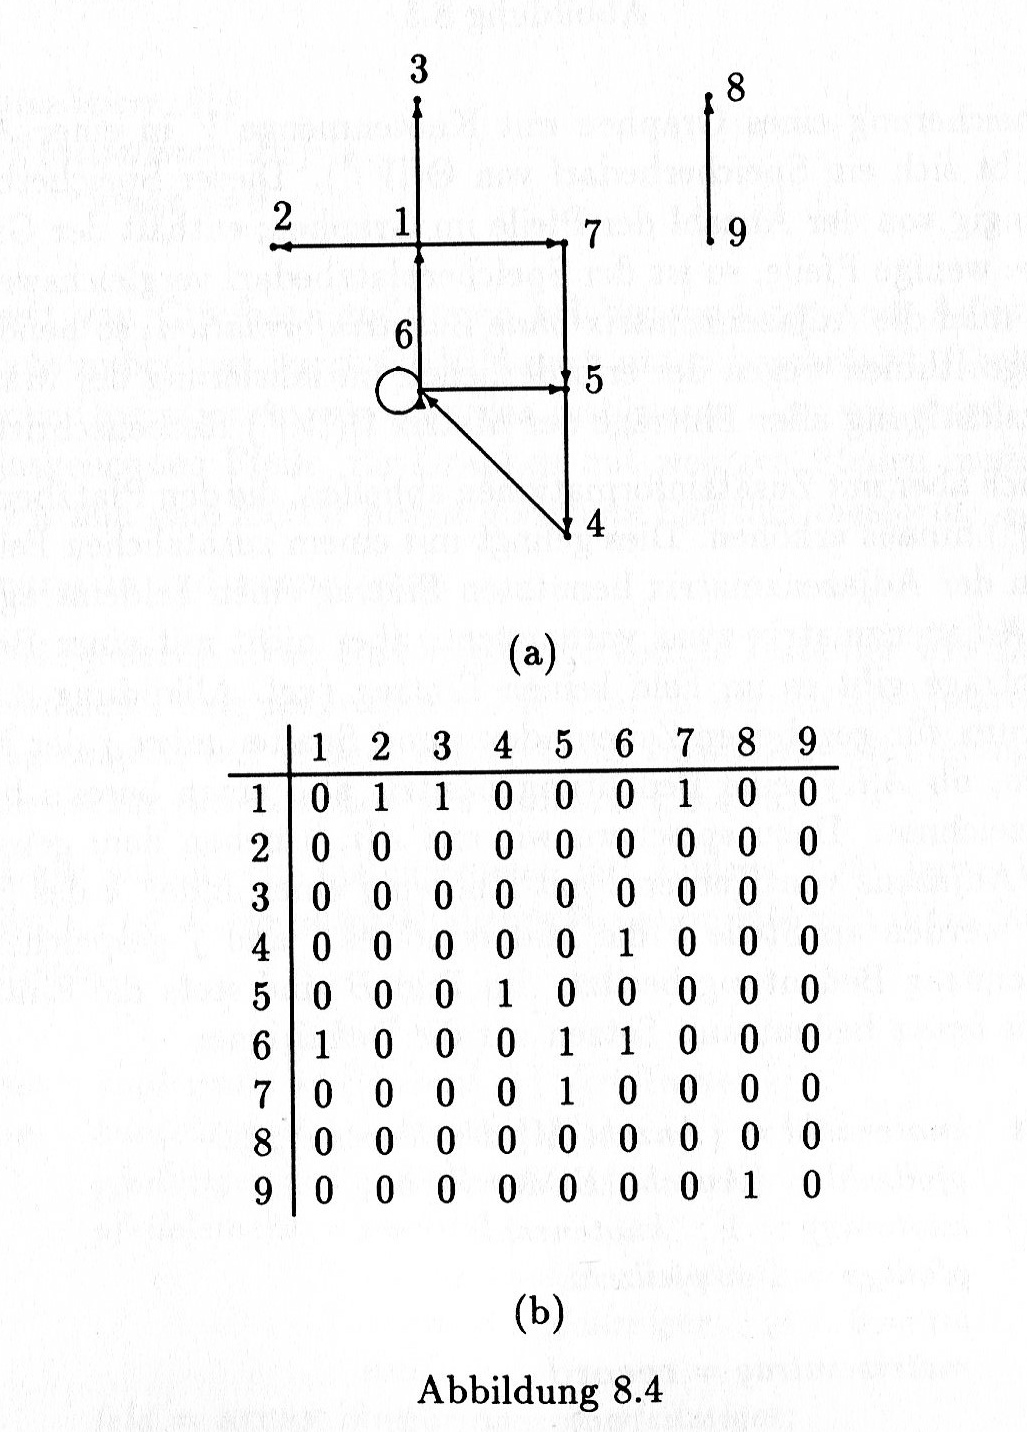
\includegraphics[width = 8cm]{./chapters/adjazenzmatrix.jpg}
\caption{Adjazenzmatrix \cite[S.539 Abb. 8.4]{OttWid90}
%{\tiny (Quelle: OTTMANN, Thomas; WIDMAYER Peter: Algorithmen und Datenstrukturen, Reihe Informatik Bd. 70, Mannheim: BI-Wissenschaftsverlag, 1990, S.539 Abb. 8.4)} 
}
\label{a2}
\end{figure}
 
\textbf{Speicherung in Adjazenzlisten}\\
Für jeden Knoten wird eine lineare, verkettete Liste seiner ausgehenden Kanten gespeichert.
Die Knoten werden als lineares Feld gespeichert (d.h. jeder Knoten im Feld zeigt auf eine Liste). \\
Dies ist effizienter als eine Adjazenzmatrix, weil kein Speicherplatz verschwendet wird.
 \footnote{vergl. Ebd., S.541-542, Speicherung in Adjazenzlisten} \\

\begin{figure}[h]
\centering
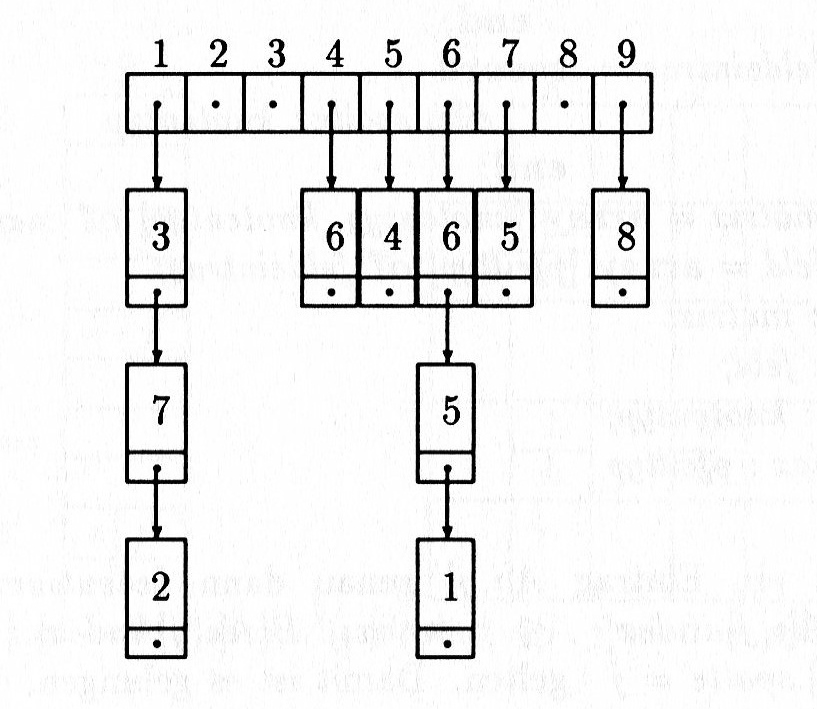
\includegraphics[width = 8cm]{./chapters/adjazenzliste.jpg}
\caption{Adjazenzliste \cite[S542 Abb 8.6]{OttWid90}
%{\tiny (Quelle: OTTMANN, Thomas; WIDMAYER Peter: Algorithmen und Datenstrukturen, Reihe Informatik Bd. 70, Mannheim: BI-Wissenschaftsverlag, 1990, S.542 Abb. 8.6)} 
}
\label{a3}
\end{figure} 

\textbf{Speicherung in doppelt verketteten Listen}\\
Jedes Element enthält Zeiger auf die beiden Nachbarelemente sowie auf eine Kantenliste (wie bei Adjazenzliste, s.o.).
Diese Darstellung besitzt die den Adjazenzlisten fehlende Dynamik, ist aber natürlich komplizierter.
 \footnote{vergl. Ebd., S.542-544, Speicherung in einer doppelt verketteten Pfeilliste}
 
\begin{figure}[h]
\centering
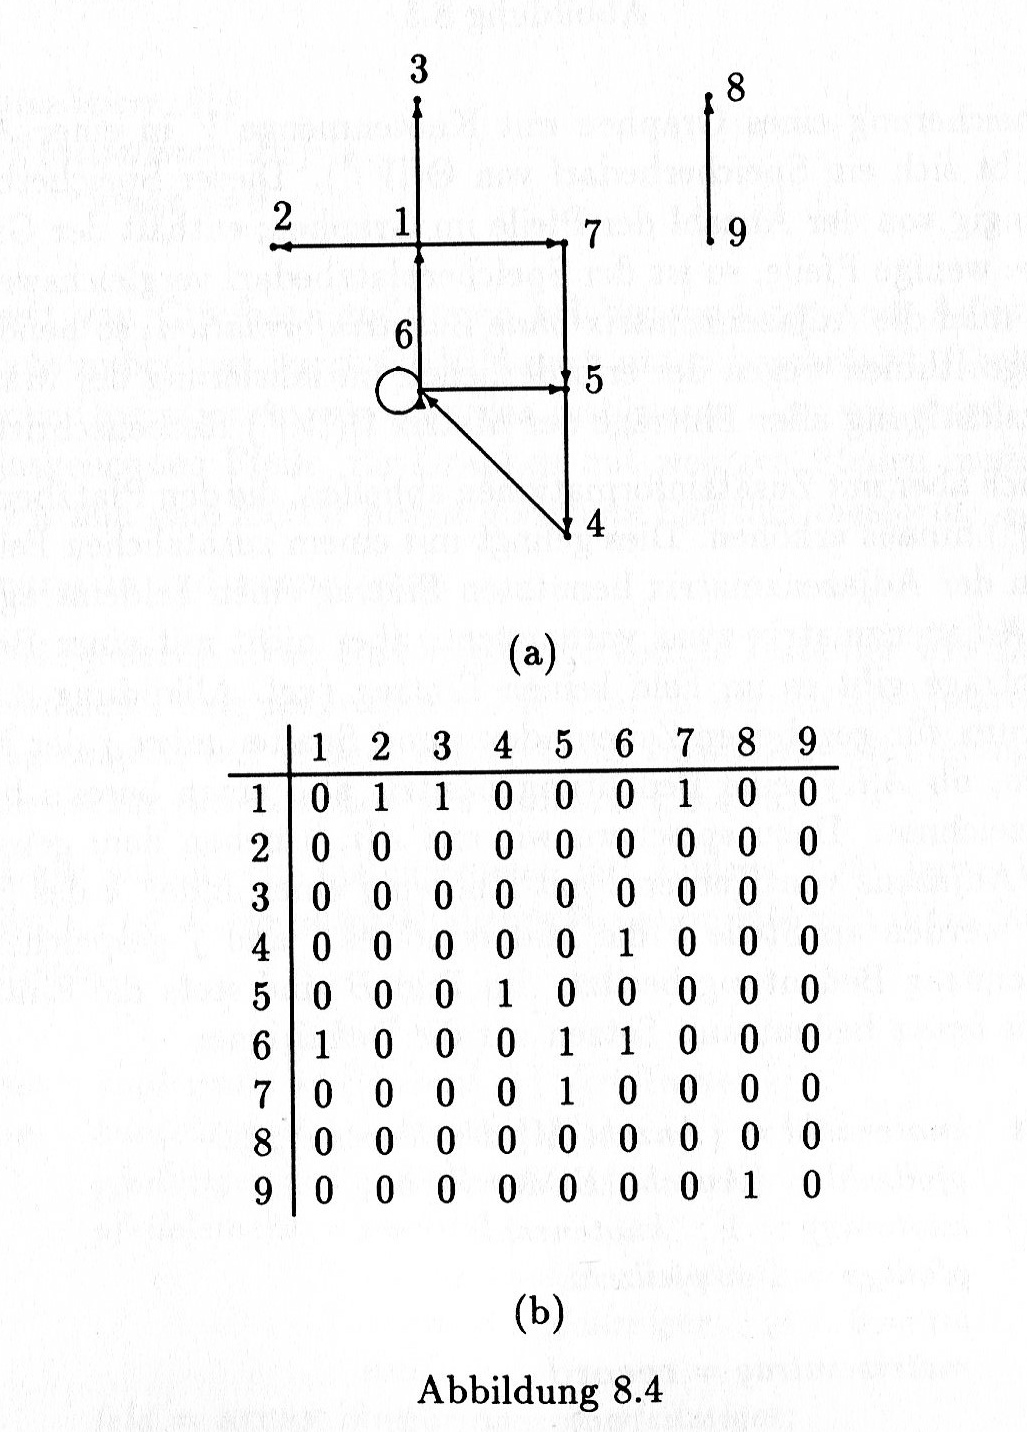
\includegraphics[width = 8cm]{./chapters/adjazenzmatrix.jpg}
\caption{doppeltVerkettetePfeilliste.jpg \cite[S.543 Abb 8.7]{OttWid90}
%{\tiny (Quelle: OTTMANN, Thomas; WIDMAYER Peter: Algorithmen und Datenstrukturen, Reihe Informatik Bd. 70, Mannheim: BI-Wissenschaftsverlag, 1990, S.543 Abb. 8.7)} 
}
\label{a4}
\end{figure}


